 \section{Evaluation}
 \label{sec:eval}


 \wajih{Use macros for common words in this whole section.}

 \wajih{Be consistent with the terminology that you used in the abstract/intro.}

 \wajih{Captions need to be lowercase}

 {\renewcommand{\arraystretch}{1.2}
 \begin{table*}[t!]
   \centering
   \footnotesize
   \caption{Comparison of \Sys against FLASH and KAIROS. Prec.: Precision; Rec.: Recall; \wajih{add what we discussed here.}}
   \setlength{\tabcolsep}{0.7pt}
   \begin{tabular}{ccccccccccccc}
     \toprule
 
   \multirow{2}{*}{\textbf{Datasets}}
   & \multicolumn{4}{c }{\Norothead{ \bf \Sys}}
   & \multicolumn{4}{c }{\Norothead{ \bf FLASH}}
   & \multicolumn{4}{c }{\Norothead{ \bf KAIROS}}
   \\ \cmidrule(r{\tbspace}){2-5} \cmidrule(r{\tbspace}){6-9} \cmidrule(r{\tbspace}){10-13}
 
     & {\bf Prec.} &  {\bf Rec.} & {\bf \fscore} & {\bf TP}/ {\bf FP}/ {\bf FN}/ {\bf TN} & {\bf Prec.}  & {\bf Rec.} & {\bf \fscore} & {\bf TP}/ {\bf FP}/ {\bf FN}/ {\bf TN} & {\bf Prec.}  & {\bf Rec.} & {\bf \fscore} & {\bf TP}/ {\bf FP}/ {\bf FN}/ {\bf TN} \\
 
   \midrule
 
   E3-CADETS &  \TCP & \TCR & \TCF & \TCTP/ \TCFP/ \TCFN/ \TCTN &  \FCP & \FCR & \FCF & \FCTP/ \FCFP/ \FCFN/ \FCTN & \KCP & \KCR & \KCF & \KCTP/ \KCFP/ \KCFN/ \KCTN \\
   E3-TRACE &  \TTP & \TTR & \TTF & \TTTP/ \TTFP/ \TTFN/ \TTTN  & \FTP & \FTR & \FTF & \FTTP/ \FTFP/ \FTFN/ \FTTN & - & - & - & - \\
   E3-THEIA &  \TTHP & \TTHR & \TTHF & \TTHTP/ \TTHFP/ \TTHFN/ \TTHTN & \FTHP & \FTHR & \FTHF & \FTHTP/ \FTHFP/ \FTHFN/ \FTHTN & \KTHP & \KTHR & \KTHF & \KTHTP/ \KTHFP/ \KTHFN/ \KTHTN \\  
   OpTC & \TOP & \TOR & \TOF & \TOTP/ \TOFP/ \TOFN/ \TOTN & \FOP & \FOR & \FOF & \FOTP/ \FOFP/ \FOFN/ \FOTN & \KOP & \KOR & \KOF & \KOTP/ \KOFP/ \KOFN/ \KOTN \\
   E5-CADETS &  \ETCP & \ETCR & \ETCF & \ETCTP/ \ETCFP/ \ETCFN/ \ETCTN  & \EKCP & \EKCR & \EKCF & \EKCTP/ \EKCFP/ \EKCFN/ \EKCTN & \EFCP & \EFCR & \EFCF & \EFCTP/ \EFCFP/ \EFCFN/ \EFCTN \\
   E5-THEIA &  \ETTHP & \ETTHR & \ETTHF & \ETTHTP/ \ETTHFP/ \ETTHFN/ \ETTHTN & \EKTHP & \EKTHR & \EKTHF & \EKTHTP/ \EKTHFP/ \EKTHFN/ \EKTHTN & \EFTHP & \EFTHR & \EFTHF & \EFTHTP/ \EFTHFP/ \EFTHFN/ \EFTHTN \\
   E5-ClearScope & \ETClP & \ETClR & \ETClF & \ETClTP/ \ETClFP/ \ETClFN/ \ETClTN  & \EKClP & \EKClR & \EKClF & \EKClTP/ \EKClFP/ \EKClFN/ \EKClTN & \EFClP & \EFClR & \EFClF & \EFClTP/ \EFClFP/ \EFClFN/ \EFClTN \\
   \bottomrule
   \end{tabular}
 \label{summary:benchmarks:large}
 \end{table*}}



We evaluate \Sys using the open-source datasets \darpa E3 and OptC, which comprise system audit logs that simulate enterprise environments. These logs are collected from both Windows and Linux operating systems. Our evaluation experiments are conducted on a machine running Ubuntu 18.04.6 LTS, equipped with an 8-core Intel CPU and 100 GB of memory. Additionally, the machine features an NVIDIA RTX2080 GPU, utilized for operating our graph learning framework. Our evaluation aims to address the following research questions (RQs).

\begin{itemize}[leftmargin=*]
\item \textbf{RQ1.} How does \Sys compares to existing systems in terms of detection performance?
\item \textbf{RQ2.} What is the effectiveness of word2vec harmonization in a utility server setting?
\item \textbf{RQ3.} What is the resource consumption of \Sys running on a client machine?
\item \textbf{RQ4.} What is the end to end processing time of \Sys on a client machine?
\item \textbf{RQ5.} How does the cost metrics of \Sys compares to centralized systems?
\item \textbf{RQ6.} How effective is the categorization based \gnnshort ensemble compared to a single \gnnshort?
%\item \textbf{RQ5.} What is the effect of varying differential privacy noise on detection performance?
\item \textbf{RQ7.} Ablation study of various \Sys components.
\end{itemize}

\subsection{Implementation}

\Sys is developed in Python in 7000 lines of code. It leverages the PyTorch and Torch Geometric libraries to implement the federated graph learning framework. For developing the \wordvec and vector harmonization module, we employ the Gensim library. Secure communication between clients and the utility server is ensured through Python's Cryptography module. All other functionalities of \Sys are encapsulated in Python functions, designed for easy customization and deployment across different system environments.


\subsection{Datasets}
%\wajih{Update it with E5}
We have utilized the \darpa E3~\cite{darpae3}, E5~\cite{darpae5}, and \optc~\cite{darpaoptc} datasets for our evaluation. The E3 and E5 datasets consist of several adversarial engagements that simulate real-world Advanced Persistent Threats on enterprise networks. In these exercises, the red team aim to exploit vulnerabilities in the enterprise's services while hiding their attacks behind benign system activities. The logs captured from these exercises are documented under various scenario names, including Cadets, Trace, and Theia.

The \optc dataset, another open-source resource from \darpa, encompasses a comprehensive collection of audit logs from an enterprise environment with 1,000 hosts. This dataset includes six days of benign system logs, serving as training data for our system to learn normal behavior patterns. Subsequently, attack logs span three days of system activities, featuring red team tactics such as initial compromises, privilege escalations, malicious software installations, and data exfiltration.

Each of these datasets is accompanied by ground truth documents that facilitate the distinction between benign and malicious events. For our evaluation, we employ attack labels from existing systems, such as \threatrace, Kairos and FLASH for our evaluation.


\subsection{Detectors for Comparison}
%\wajih{Add citations. Say a few lines about the PIDS that we do not compare against. Read Kairos evaluation section -- they have very good sentences about why they don't compare against several existing PIDS. Make sure that you do not miss any PIDS system. Make sure to cite this paper: https://www.usenix.org/system/files/sec23winter-prepub-490-jia.pdf}

To benchmark our system, we conduct comparisons against existing state-of-the-art Provenance-based Intrusion Detection Systems (PIDS). \threatrace~\cite{wang2022threatrace}, a node-level system, employs graph representation learning to identify anomalous nodes within a provenance graph. In contrast, FLASH~\cite{flash2024}, another node-level system, outperforms \threatrace in both detection efficiency and effectiveness by leveraging semantic feature vectors and an embeddings database. Given FLASH's superiority over \threatrace, our comparison primarily focuses on FLASH. Additionally, we include KAIROS~\cite{cheng2023kairos} in our comparison, which utilizes temporal graph networks to capture the evolution of a system's provenance graph over time. We do not compare against Streamspot~\cite{streamspot} and Unicorn~\cite{han2020unicorn} as they are graph-level detectors, and recent systems like \threatrace and FLASH have been shown to surpass them in detection performance. While DISTDET~\cite{dong2023distdet}, Prographer~\cite{yangprographer} and Shadewatcher~\cite{shadewatcher} are notable PIDSes, we exclude them from our comparison because DISTDET, Prographer is closed-source and a major component of Shadewatcher is proprietary, which hinders our ability to conduct a thorough comparison.

 \subsection{Detection Performance}

 %\wajih{do not start each paragraph by saying "In this section"...}
 We conducted experiments to assess how \Sys compares with other systems in terms of detection performance. Initially, we outline our methodology for deploying \Sys on the \darpa E3, E5, and \optc datasets. The E3 dataset comprises various scenarios, including Cadets, Theia, and Trace, each representing logs generated by a single host machine. To evaluate \Sys on E3, we treat each scenario as an individual host. Consequently, in our federated learning approach, we trained local \gnnshort models on each scenario individually. These local models then participated in federated averaging, a process repeated across \textit{K} rounds. Upon completing the training, we evaluated the global \gnnshort model against the attack logs from these E3 scenarios. Similar to E3, the E5 dataset is also divided into different scenarios; however, each scenario comprises three different hosts. For each scenario, we use benign logs data from these different hosts to train our system and then evaluate it on the attack logs. For the \optc dataset, which is divided among a thousand hosts, we sampled \textit{N} hosts for inclusion in our federated graph learning experiment. Additionally, we conducted experiments with a varying number of randomly selected hosts, the results of which are detailed in our ablation study. For conducting these evaluations, we use the same detection metrics as defined by existing node-level detectors such as \threatrace and FLASH.

 Table~\ref{summary:benchmarks:large} reveals that \Sys's performance on these datasets is comparable to that of FLASH, despite the diverse log patterns and information contained within each E3, E5, and \optc client. This underscores \Sys's capability to maintain robust detection performance amidst such heterogeneity. KAIROS's evaluation, based on a coarser time-window granularity compared to the node-level granularity of FLASH and \Sys, poses a challenge for direct comparison. Nevertheless, our results remain competitive with KAIROS.
 
 Beyond detection performance, we also highlight \Sys's qualitative advantages, including its privacy-preserving features and distributed, scalable operation. These aspects underscore the value of \Sys in contrast to more centralized systems, emphasizing its utility in a broader range of applications.

\subsection{Effectiveness of Categorized Graph Learning}

To examine the effectiveness of our process categorization based \gnnshort ensemble technique, we conducted experiments comparing our ensemble approach against a single model approach. Specifically, for the ensemble method, we designated the number of categories to be 10. This approach standardizes all processes across various hosts into 10 distinct categories, ensuring that the \gnnshort models learn similar distributions regardless of the host. Such standardization is crucial for mitigating the impact of heterogeneous distributions during the federated averaging process. Table~\ref{categorized_gnn} presents the experimental outcomes on the \darpa E3 and \optc datasets. The results indicate that utilizing categorized ensemble models yields superior performance. This improvement is attributed to each sub-model's enhanced ability to concentrate on different patterns of system activity, thereby reducing the likelihood of these patterns becoming conflated during the federated averaging process.

\begin{table}[t!]
  \centering
  \small
  \setlength{\tabcolsep}{10pt}
  \caption{Effectiveness of categorized \gnnshort learning.}
  \begin{tabular}{ | c | c | c | c | c |}
    \hline
    \bf Dataset & \bf Type & \bf Prec. & \bf Rec. & \bf \fscore \\
    \hline
    \multirow{2}{*}{E3-Cadets} & Single & \STCP & \STCR & \STCF \\ 
    \cline{2-5} 
    & Ensemble & \TCP & \TCR & \TCF \\
    \hline
    \multirow{2}{*}{E3-Trace} & Single & \STTP & \STTR & \STTF \\
    \cline{2-5} 
    & Ensemble & \TTP & \TTR & \TTF \\
    \hline
    \multirow{2}{*}{E3-Theia} & Single & \STTHP & \STTHR & \STTHF \\
    \cline{2-5} 
    & Ensemble & \TTHP & \TTHR & \TTHF \\
    \hline
    \multirow{2}{*}{\optc} & Single & \STOP & \STOR & \STOF \\
    \cline{2-5} 
    & Ensemble & \TOP & \TOR & \TOF \\
    \hline
  \end{tabular}
  \label{categorized_gnn}
\end{table}

 \subsection{Efficacy of Word2vec harmonization}

 \wajih{never use !h instead use !t in the table layout. Same rule goes for figures. Exception to this rule is Appendix.}
 \begin{table}[h!]
  \centering
  \small
  \setlength{\tabcolsep}{3.5pt}
    \caption{Effectiveness of \wordvec vectors harmonization. }
      \begin{tabular}{ | c | c | c | c | c | c |}
        \hline
          \bf Word2vec Type & \bf Precision & \bf Recall & \bf \fscore & \bf TP & \bf FP \\
        \hline
         Local & \VFOP & \VFOR & \VFOF & \VFOTP & \VFOFP \\
         \hline
         Harmonized & \TOP & \TOR & \TOF & \TOTP & \TOFP \\
        \hline
      \end{tabular}
      \label{local:wordvec}
  \end{table}

 We evaluated the effectiveness of our Word2Vec vector harmonization scheme through two experiments using the \optc dataset. In the first experiment, each client utilized its locally trained Word2Vec model to encode semantic features during the training process. In the second experiment, we synchronized the individually trained models into a central Word2Vec model using the utility server architecture, as explained in Section~\ref{sec:methodology}. Then each client used this centralized model for generating semantic features. Table~\ref{local:wordvec} presents the experimental results. By employing the harmonized models, we achieved significantly better detection outcomes. This improvement is attributable to the inherent randomness of the Word2Vec algorithm, which causes different clients to produce divergent vectors for identical attributes. Such variability leads to heterogeneity in the feature vectors for the \gnnshort model, impairing the model's ability to generalize and converge effectively during the federated learning process, thereby yielding suboptimal results. However, through our novel, privacy-preserving aggregation of these semantic models, we have addressed this issue.

 \subsection{Resource Consumption}

 We used different batches of audit events of varying sizes to model the resource utilization on a client machine comprehensively. The results, as depicted in Figure~\ref{fig:resource}, indicate that the resource consumption of \Sys is moderate. Specifically, \Sys is capable of processing up to 100,000 audit events simultaneously while consuming less than 900 MB of memory and utilizing less than 20\% of CPU resources. This suggests that \Sys does not significantly burden the client machine, particularly given that client machines typically experience low event throughput. Consequently, our system requires execution only a few times per day to process newly accumulated events, implying that resource consumption is not continuous but occurs at specific intervals. Furthermore, our analysis of the host data in the \optc dataset reveals that, on average, each client generates approximately 100,000 audit log events within a three-hour period.

 \begin{figure}[t!]
  \centering
  \subfloat[CPU utilization.]{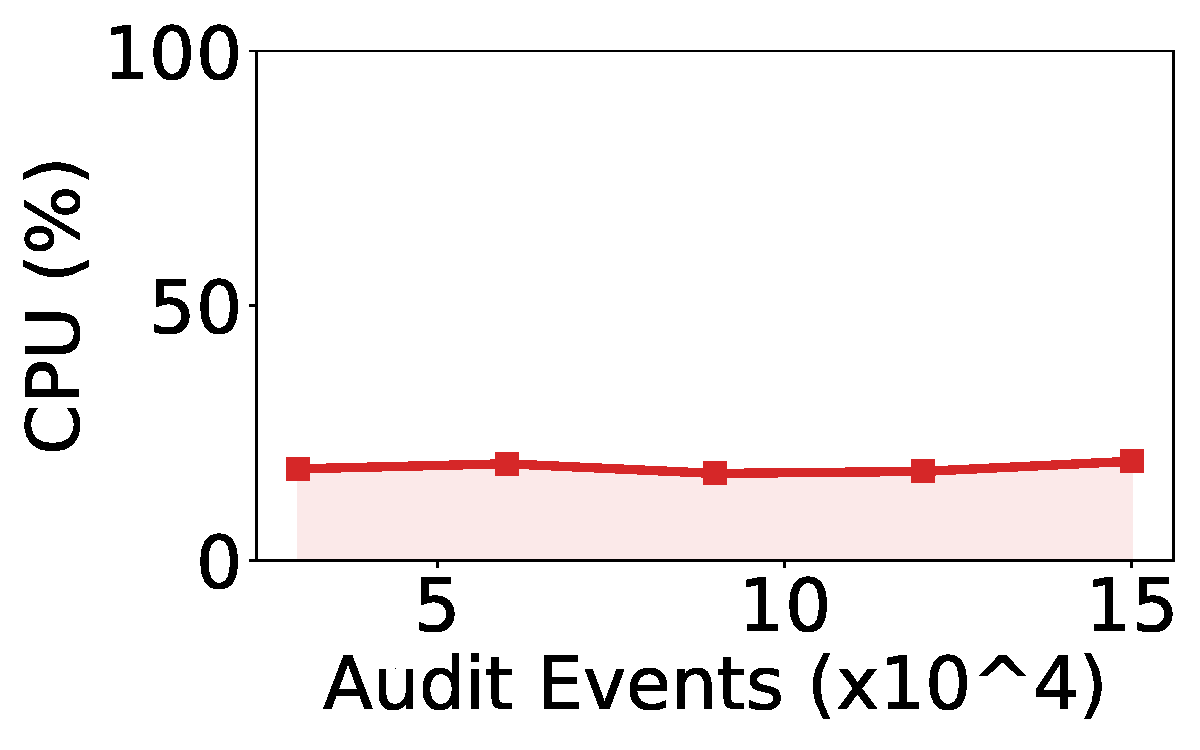
\includegraphics[width=0.24\textwidth]{fig/cpu.pdf}\label{cpu}}
  \hfill
  \subfloat[RAM utilization]{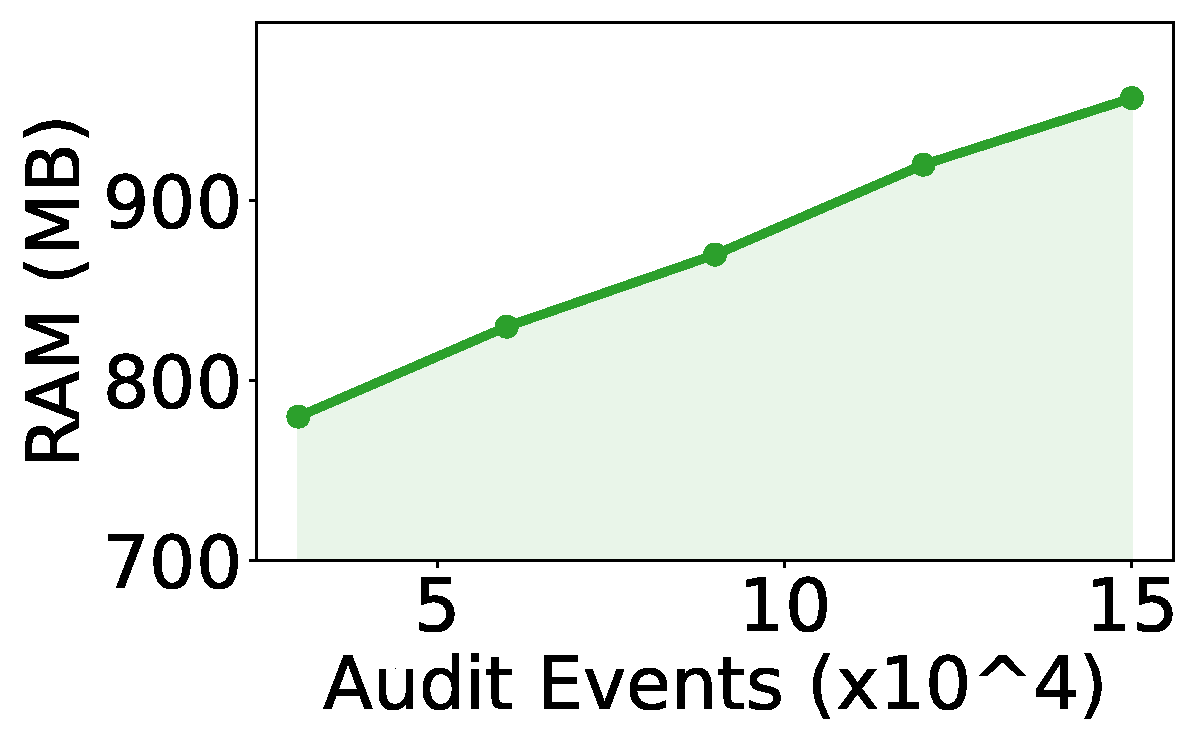
\includegraphics[width=0.24\textwidth]{fig/ram.pdf}\label{ram}}
  \hfill
  \caption{Resource consumption of \Sys evaluated using \optc dataset.}
  \label{fig:resource}
  \vspace{-2ex}
\end{figure}

 \subsection{Processing Time Analysis}

 We conducted experiments to study the end-to-end processing time of our system. For this, we used batches of audit events of various sizes, conducting end-to-end inference with \Sys to measure the time taken to process these events on a client machine. The results, illustrated in Figure~\ref{sizevstime}, demonstrate that \Sys processes events with notable efficiency. For example, it requires approximately 23 seconds to process a batch of 100,000 events. Given our previous analysis of host logs in the \optc dataset, which indicated that each host generates an average of 100,000 events in three hours, \Sys can process 24 hours worth of log data on a client in merely 3 minutes. This level of efficiency ensures that our system is highly effective, preventing any potential log congestion.

 \begin{figure}[t!]
  \centering
  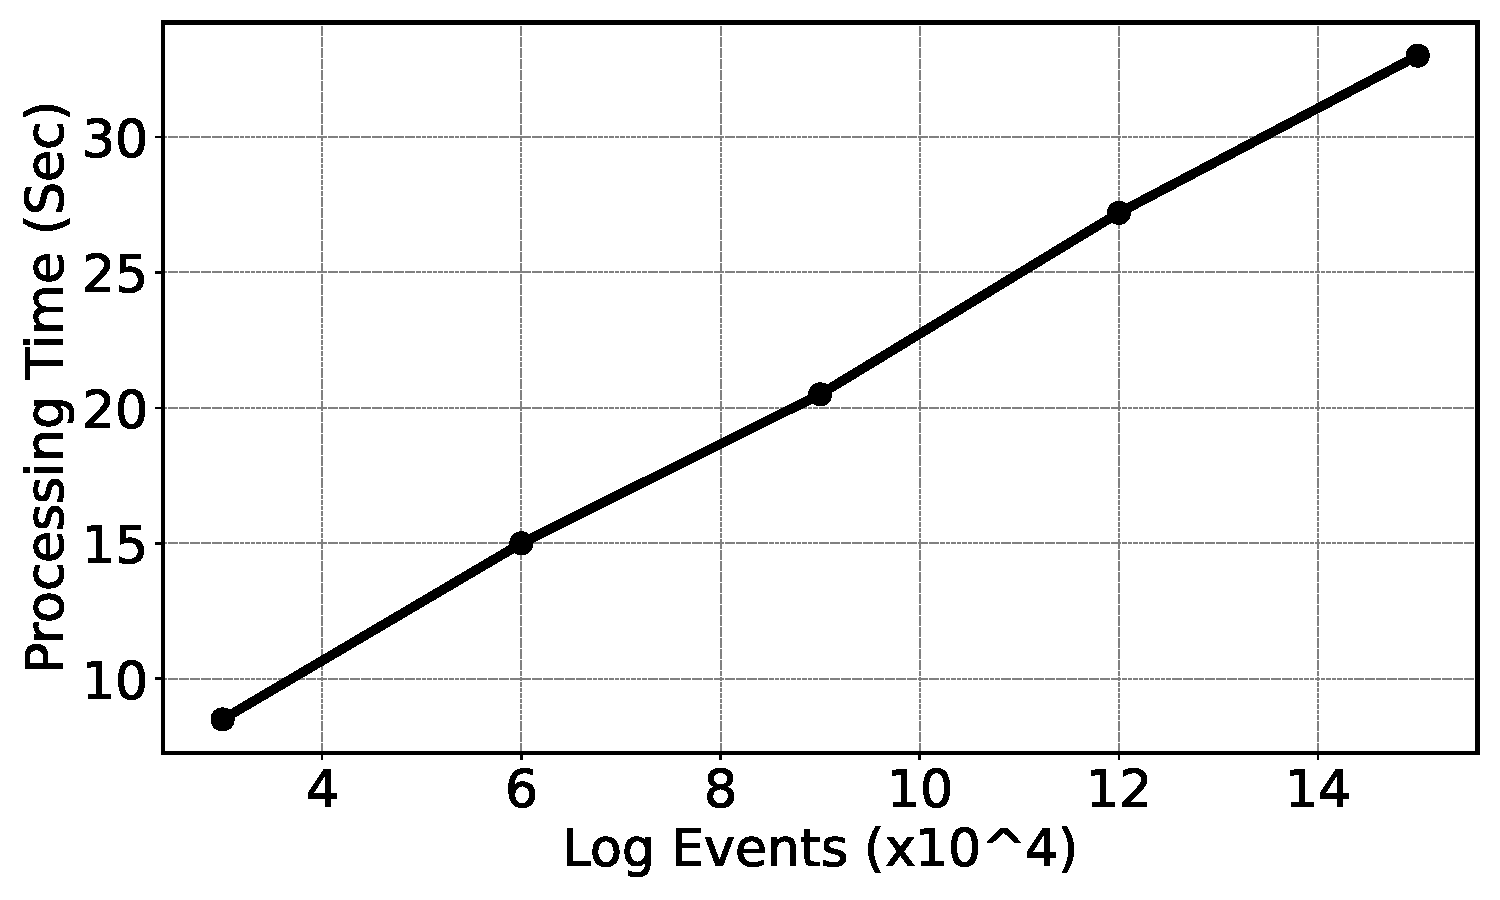
\includegraphics[width=0.4\textwidth]{fig/sizevstime.pdf}
  \caption{Processing time for various audit event sizes evaluated using \optc dataset.}
  \label{sizevstime}
  \vspace{-2ex}
\end{figure}

%  \subsection{Effect of Local Differential Privacy}

%  \begin{figure}[t!]
%   \centering
%   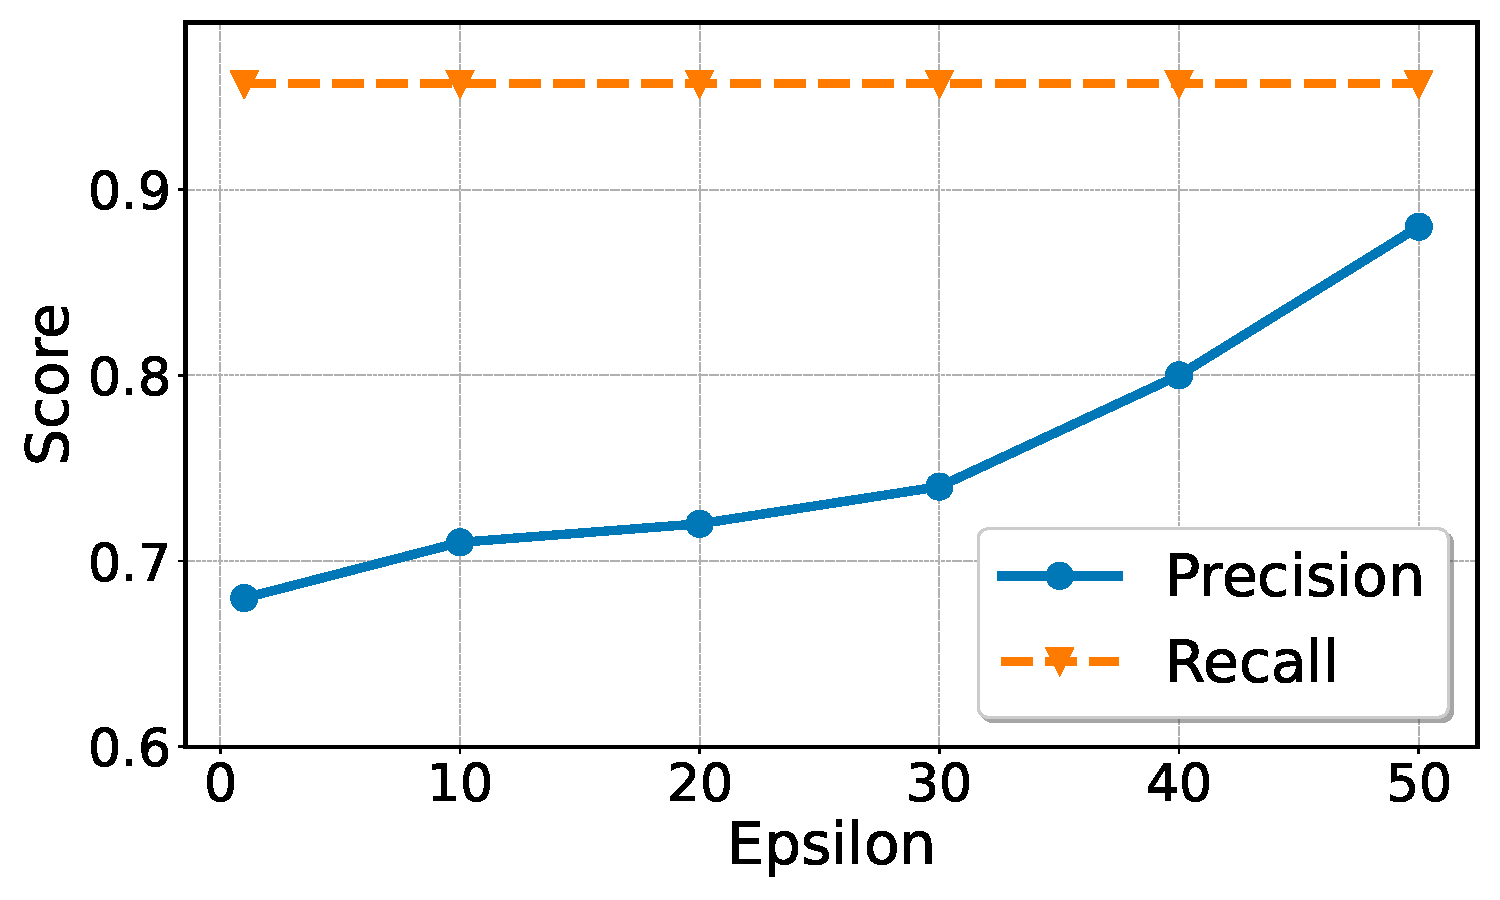
\includegraphics[width=0.48\textwidth]{fig/epsvsscore.pdf}
%   \caption{Effect of Epsilon ($\epsilon$) on Detection Performance.}
%   \label{epsvsscore}
%   \vspace{-2ex}
% \end{figure}

%  In this section, we examine the impact of differential privacy noise levels on the detection performance of \Sys. Differential privacy introduces a parameter, $\epsilon$, which dictates the intensity of Gaussian noise added to the local \gnnshort model updates prior to their aggregation at the central server for federated averaging, as detailed in Section~\ref{sec:methodology}. By adjusting $\epsilon$ during the training phase, we assess the detection capabilities of the globally trained model across various $\epsilon$ settings. Figure~\ref{epsvsscore} illustrates the relationship between $\epsilon$ and detection performance. It is important to note that lower $\epsilon$ values correspond to higher noise levels in model updates, thereby strengthening privacy at the expense of model utility. Conversely, increasing $\epsilon$ reduces noise strength, improving detection performance. The optimal $\epsilon$ value is contingent upon the specific requirements and context of the organization employing \Sys, balancing between privacy protection and model utility.

\subsection{Cost Metric Analysis}
\label{cost_metric}
We examined the operational costs of deploying \Sys in comparison to centralized solutions like FLASH and KAIROS for organizational use. Our evaluation concentrates on three primary cost components: network expenses (\(C_{N}\)), the cost of storing raw data (\(C_{S}\)), and processing costs (\(C_{P}\)).

To begin, we estimate these costs for the FLASH system utilizing the \optc dataset. Each host within \optc produces approximately 1GB of audit logs daily, equating to nearly one million audit events. For an organization with 1,000 hosts, the total daily log volume would be 1,000 GB. This data volume requires transmission over the network and storage on a central server operating FLASH. Additionally, FLASH processes one million events in about 100 seconds, implying that processing events from 1,000 clients would necessitate approximately 27.7 hours. In contrast, KAIROS processes 57,000 events in 11.6 seconds, leading to a processing time of 204 seconds for one million events. Consequently, processing data from 1,000 clients with KAIROS would require around 56.6 hours.

To calculate the daily operational costs of running these systems for a specific organization, we utilized the Google Cloud Platform's (GCP) pricing calculator~\cite{gcp}. The cost to operate FLASH under the previously mentioned workload is estimated at \$135, with computing expenses accounting for \$100 and storage and network costs comprising \$35. Given its longer processing duration, the operational cost for KAIROS would be twice that of FLASH.

Compared to existing systems, \Sys processes client logs in a federated manner, eliminating the need for logs to leave the client's machine. The only network expenses arise from the transmission of \gnnshort and Word2Vec models. Specifically, the \gnnshort model is 13kb, while the average Word2Vec model is 6 MB. For an organization with 1,000 hosts, the communication cost with the central server would be 12.70 MB, and for the utility server, it would be 5.86 GB. Overall, \Sys achieves a 170-fold reduction in communication and storage costs compared to FLASH and Kairos. The central and utility servers conduct a simple mean operation on the models, taking only a few seconds. Therefore, the operational cost of \Sys for 1,000 client machines is approximately \$10 per day, marking a 13-fold reduction compared to FLASH and a 26-fold reduction compared to Kairos.

 \subsection{Ablation Study}

 In this ablation study, we analyze the impact of key parameters within \Sys. Specifically, we focus on two principal parameters: $N$, representing the number of client machines participating in Federated Graph Learning, and $R$, denoting the number of rounds the federated averaging process is executed. The effect of these parameters is discussed below: \\

\PP{Hosts vs Detection Performance} We utilized the \optc dataset for this experiment, randomly selecting a variable number of hosts to participate in training our model through federated learning. The trained global model was then applied to perform threat detection, with the outcomes documented accordingly. Figure~\ref{scoresvshosts} presents these results, illustrating that performance improvement is observed up to a certain number of hosts. This plateau is attributed to the \optc dataset's finite set of benign patterns that can be learned. Beyond this threshold, additional hosts do not contribute new information beneficial to the model, thus halting further performance gains and increasing the risk of overfitting. To mitigate this, client machines can monitor and report the loss of the global model on their local datasets, providing a metric for the server to determine the optimal point to cease the learning process. \\

\begin{figure}[t!]
  \centering
  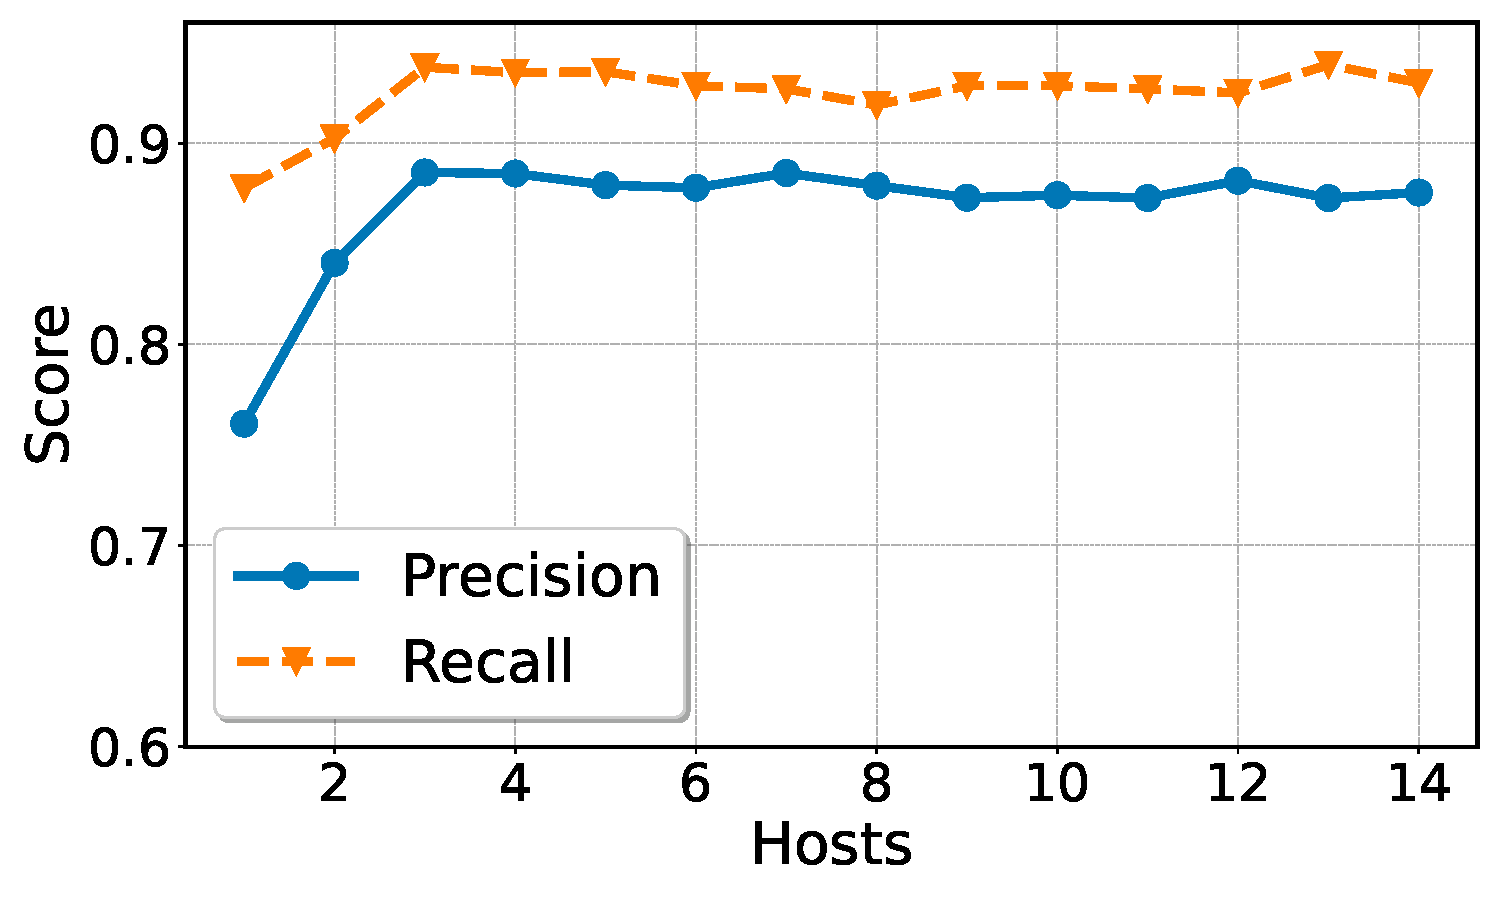
\includegraphics[width=0.4\textwidth]{fig/scoresvshosts.pdf}
  \caption{Effect of number of hosts vs detection metrics.}
  \label{scoresvshosts}
  \vspace{-2ex}
\end{figure}

\PP{Effect of Federated Averaging Rounds} We employed the \darpa E3 dataset to examine the impact of federated averaging rounds on detection performance. Our methodology involved training the model over a range of federated averaging rounds and subsequently evaluating the model's detection capabilities. The outcomes are depicted in Figure~\ref{roundsvsscore}, which shows that detection performance improves up to a certain number of rounds before declining due to overfitting. Notably, this inflection point is also characterized by a minimal decrease in training loss, suggesting that the model has reached its learning capacity. This observation proves to be a valuable metric for determining the optimal moment to stop training, thereby preventing overfitting and ensuring optimal model performance.

\begin{figure}[t!]
  \centering
  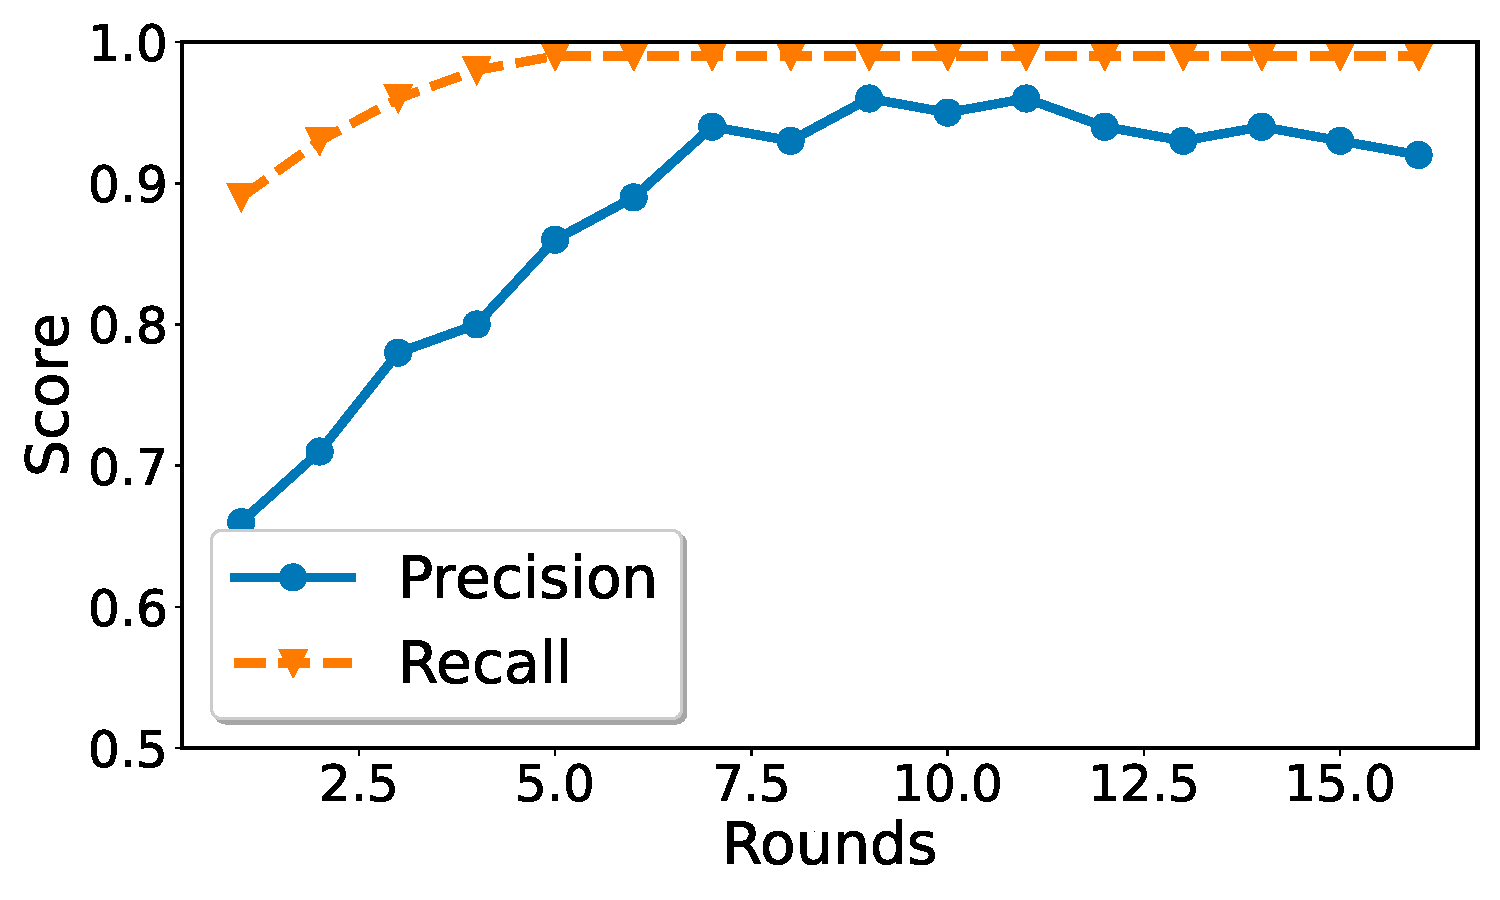
\includegraphics[width=0.4\textwidth]{fig/roundsvsscore.pdf}
  \caption{Federated averaging rounds vs detection performance. \wajih{there is no need to capitalize every word in the caption. It applies to other figures as well.}}
  \label{roundsvsscore}
  \vspace{-2ex}
\end{figure}

\PP{Effect number of categories vs Detection} We studied the impact of varying the number of categories ($K$) on the performance of detection. Within our entity-level personalized \gnnshort learning framework, $K$ dictates the creation of distinct standardized bins. These bins categorize processes across client machines. Subsequently, we employ an ensemble approach, deploying a separate GNN model for each bin. Thus, the total number of GNN models corresponds to the number of categories. The results depicted in Figure~\ref{catgvsscore} indicate that an increase in $K$ enhances precision while maintaining recall levels. This outcome arises because a single model suffices for achieving high recall by effectively distinguishing between benign and malicious patterns. Nevertheless, a solitary model falls short in fully generalizing across the diverse benign patterns unique to each client due to the potential blending of individual patterns during the process of federated averaging. Employing a specialized GNN strategy across various categories addresses this challenge by minimizing false alarms.

\begin{figure}[t!]
  \centering
  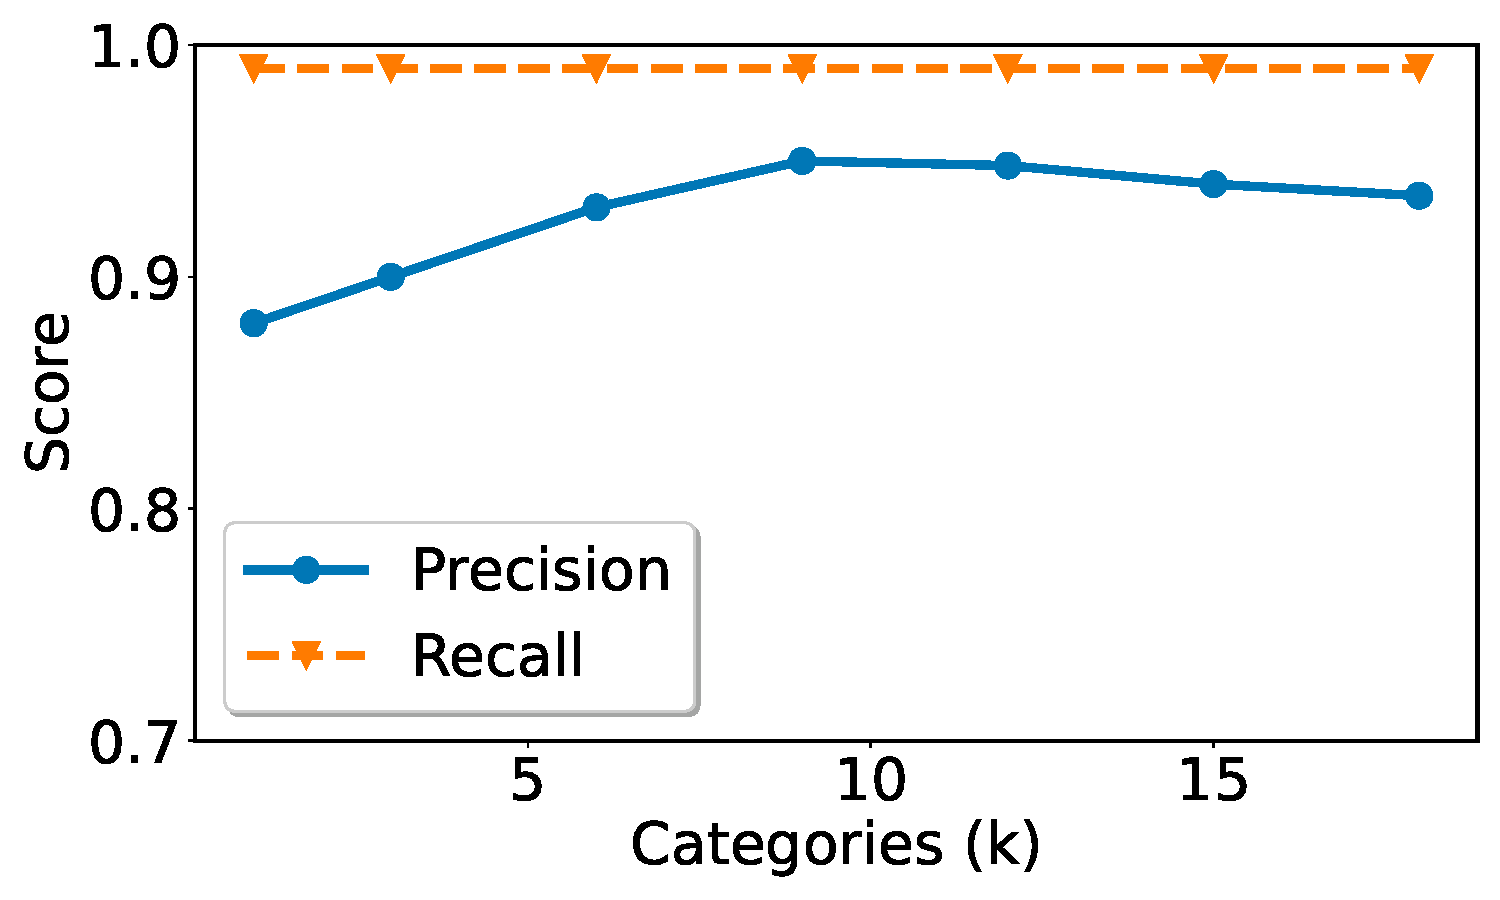
\includegraphics[width=0.4\textwidth]{fig/kvsscore.pdf}
  \caption{Number of categories vs detection performance.}
  \label{catgvsscore}
  \vspace{-2ex}
\end{figure}

\subsection{Detection Performance Under Different Methods}

\wajih{In the Nature's paper they apply different federated learning and GNN approaches to show that the one they propose is best. I remember you tried different FL approaches as well. Also tried if you can replace GNN with something else. In our Flash paper we have something similar where we switched ML methods to show the performance. I would like to see similar experimentation here as well. The idea is to prove that the method that we chose is the best.}

\subsection{Adding more clients}

\wajih{How \Sys's performance and resource consumption scale with the size of the deployed environment?  Evaluating the system's scalability by incrementally increasing the number of nodes}

% \begin{figure}[t!]
%   \centering
%   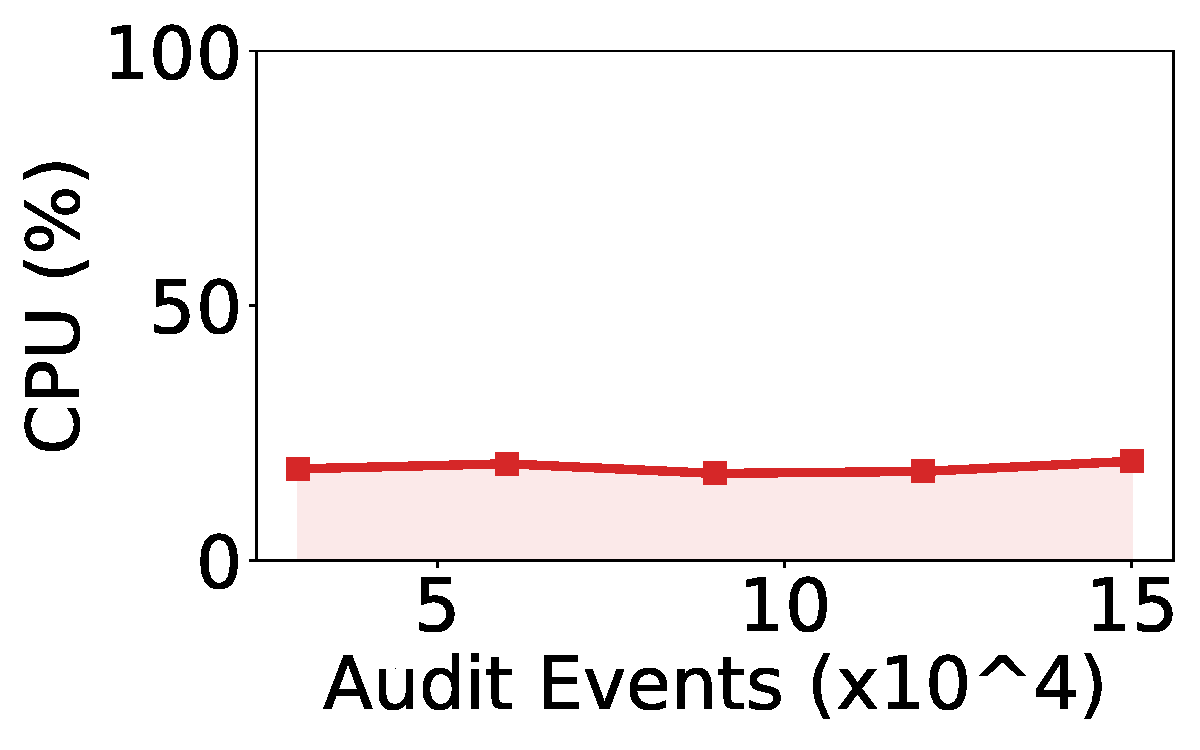
\includegraphics[width=0.40\textwidth]{fig/cpu.pdf}
%   \caption{CPU Usage}
%   \label{cpu}
%   \vspace{-2ex}
% \end{figure}

% \begin{figure}[t!]
%   \centering
%   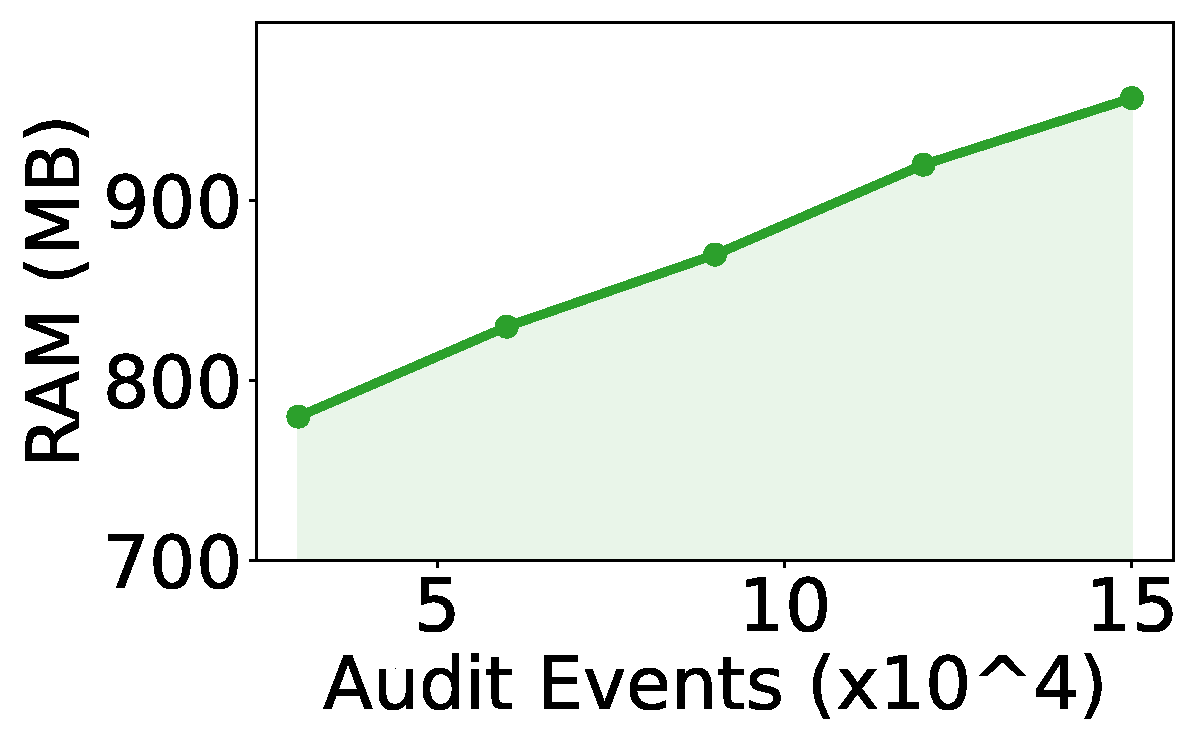
\includegraphics[width=0.40\textwidth]{fig/ram.pdf}
%   \caption{RAM usage}
%   \label{ram}
%   \vspace{-2ex}
% \end{figure}